\chapter{Vector boson scattering in the standard model and beyond}
\label{ch:phenomenology}
The particle content of the SM was established through decades of
observations of radioactive decays, cosmic rays, and particle
collisions at accelerators, as discussed in Chapter~\ref{ch:introduction}. 
To the best of our
current knowledge, all collisions at the LHC involve only these objects,
interacting via the known forces.
However, there are tantalizing hints of additional particle content and the 
interactions based on cosmological observations, which suggest a ``dark matter''
that interacts gravitationally but not electromagnetically. In addition, 
the fact that the SM does not exclude additional particles or interactions at
higher energy scales is sufficient motivation to look for them. Due to the success
of the SM in describing our current set of observations, we expect these
``new physics'' modifications to respect our current observations.
This chapter introduces the mathematical formalism of the SM, and possible
extensions that are probed by the experimental results of this thesis.

\section{Mathematical formalism of the standard model}

Through these experimental tests and
discoveries, we have also built a description of all the known interactions 
of the SM particles in the language of gauge quantum field theory (QFT).
Particles in QFT arise as excitations in quantum fields.
The equations of motion and interactions for the quantum fields of the SM can
be extracted from the SM Lagrangian, which can be divided in to 
terms governing the propagation of free fields of the spin $1/2$ fermions,
the quarks and leptons, the spin 0 Higgs field, and the gauge fields:
\begin{equation}
  \mathcal{L}_{SM} = \mathcal{L}_{\text{gauge}} + \mathcal{L}_{\text{leptons}} + 
      \mathcal{L}_{\text{quarks}} + \mathcal{L}_{\text{scalar}} \,.
  \label{eq:smlagrangian}
\end{equation}
In this expression, $\mathcal{L}_{\text{gauge}}$ is a function of the 
spin 1 gauge fields---$G_a$, associated with the gluons of the strong
force, and $A_\mu$ and $\mathbf{b_{mu}}$, associated with the electroweak force.
The $\mathcal{L}_{\text{quark}}$ includes kinetic terms describing the 
propagation of free quarks as well as interaction terms coupling the quarks
to the gluon, $A_\mu$, and $\mathbf{b_\mu}$ fields. 
The term $\mathcal{L}_{\text{quarks}}$ is built from similar kinetic terms and 
interaction terms coupling the leptons to the electroweak fields, reflecting
the fact that the leptons do not participate in the strong interaction.

A fundamental property of the SM Lagrangian is its invariance 
under under so-called ``gauge transformations,'' in which a transformation 
of the fermion fields and the associated gauge field result in a mathematically
identical Lagrangian. The full SM Lagrangian respects transformations of the
group $\SUthree_C \bigotimes\SUtwo_L\bigotimes \Uone_Y$. 
In this expression, $\SUthree$ ($\SUtwo$) is the Lie group of all two-by-two
(three-by-three) matrices with determinant 1, and $\Uone$ is the Lie group
of complex numbers. The subscripts $C$, $L$, and $Y$ indicate the fermion
and gauge fields that are impacted by the rotation: the $\SUthree$ transformation
concerns only objects with color charge (quarks and gluons), and the $\SUtwo$
and $\Uone$ rotations concern weak isospin charge, which is carried only by 
the left-handed fermions, and weak hypercharge.

The measurements in this thesis are probe the structure of the gauge term
associated with the electroweak force. 

Follow the Quigg article to give some specifics for the EW force

\section{Electroweak symmetry breaking}

\section{Particle scattering and perturbative calculations}

Together with the principle of least action, the SM Lagrangian 
can be used to to derive the equations of motion of the SM fields. For the kinetic
terms, exact solutions can be obtained, however, closed-form equations of motion
do not exist when the interaction terms are also relevant.
The strength of these interaction is set by the coupling constants $g_i$
associated with the gauge fields, as described for the electroweak interaction
in Equations~\ref{}. If the couplings, and therefore the interactions, can be 
considered small, they can be treated as a perturbation of the free-field
propagation. Because field interactions are local, associated with 
a range of the interaction communicated by the gauge field,
this treatment is particularly well suited for scattering experiments.
Free, non-interacting fields are brought together in collision 
from a large separation, where the distance scale of the interacting fields
is proportional to the energy of the collision. After interaction,
free fields, possibly of different type than those brought to collision,
emanate from the interaction point.

\begin{figure}[htbp]
  \centering
   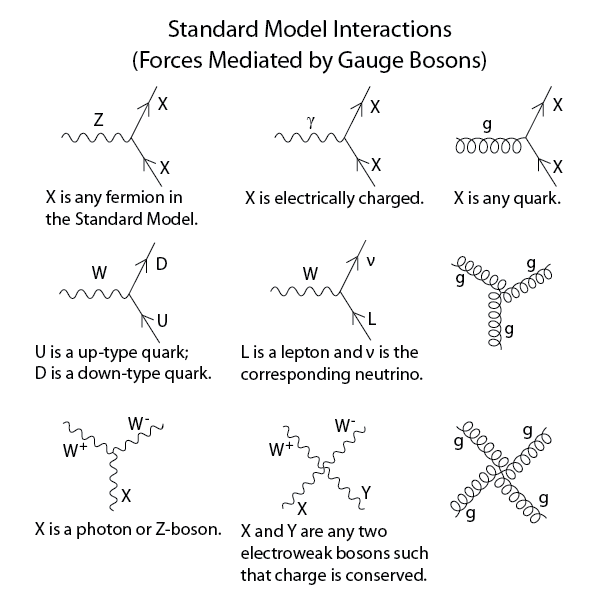
\includegraphics[width=0.7\textwidth]{figures/Phenomenology/Standard_Model_Feynman_Diagram_Vertices.png}
  \caption[Interactions allowed in the SM, excluding those involving the Higgs field]{
    Interactions allowed in the SM, excluding those involving the Higgs field.
    Reproduced from Ref.~\cite{Smith:2646356}.
        }
 \label{fig:SMinteractions}
\end{figure}

The allowed interactions in the SM are illustrated in Fig.~\ref{fig:SMinteractions}. Lines represent
propagating fields, and vertices represent interactions, arising from the
interaction terms in the SM Lagrangian. These illustrations,
known as Feynman diagrams, can be pieced together to give a diagrammatic
picture of a scattering interaction. Fig.~\ref{fig:wz3lfeynman} shows
an example quark-quark interaction---which contributions to $\pp$ collision
at the LHC---mediated by the $\PW$ and $\PZ$
bosons, leading to free muon, electron, and electron neutrino fields. 

\begin{figure}[htbp]
  \centering
   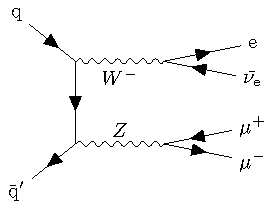
\includegraphics[width=0.4\textwidth]{figures/FeynmanDiagrams/WZ3lfeynman.pdf}
   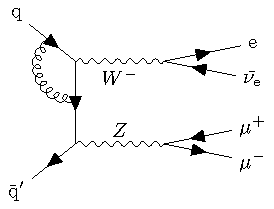
\includegraphics[width=0.4\textwidth]{figures/FeynmanDiagrams/WZ3lNLOfeynman.pdf}
  \caption{
    Feynman diagrams illustrating the $\Pq\Paq\to\mathrm{e}\PAGne\MM$ process,
    proceeding via quark and lepton couplings to the $\PW$ and $\PZ$ bosons.
        }
 \label{fig:wz3lfeynman}
\end{figure}

Feynman diagrams are not just useful as an illustration, they 
represent terms in the perturbative expansion used to model
interactions, specifically, elements of the scattering matrix that 
connects the initial and final state in a scattering experiment. 
So-called Feynman rules
are used to associate the fields and interactions of a diagram with the mathematical
formalism, giving mathematical expressions for the matrix elements
connecting the outgoing particle
four momenta and quantum numbers to the incoming particle properties.
Observables, including the total
rate of production for a final state given the initial state, are dependent
on the square of the scattering matrix elements.

The diagram in Fig.~\ref{fig:wz3lfeynman} (left) is not the only possible
set of interactions connecting the $\Pq\Paq$ initial state to the
$\mathrm{e}\PAGne\Paq\MM$ state. Other contributions include
diagrams where the $\PW$ and $\PZ$ bosons couple directly. In addition,
more intricate arrangements of the quark and gluon lines are possible,
as shown in Fig.~\ref{fig:wz3lfeynman} (right). A critical difference in
these two contributions to the $\Pq\Paq\to\mathrm{e}\PAGne\Paq\MM$ process is the
number of vertices, which contribute additional factors of the EW and
QCD couplings. If this coupling term is $\ll$1, the dominant contribution
will come from diagrams such as Fig.~\ref{fig:wz3lfeynman} (left), and
it may be possible to neglect the contribution of Fig.~\ref{fig:wz3lfeynman} (right).
Perturbative calculations rely on this approximation
by restricting a calculation to a maximum ``order'' $\mathcal{O}(\alpha^{n})$ 
in the coupling $\alpha \propto g^2$, by only considering
contributions to a process that have at most a dependence $\alpha^{n}$.

While the diagram in Fig.~\ref{} (right) does produce $\mathrm{e}\PAGne\Paq\MM$,
it does so with an additional gluon. It is tempting to consider this as a separate
process, however, due to the nature of the strong force, such an approach is not favorable experimentally.
Free gluons are not observable, rather, they hadronize into baryons and mesons.
In addition, 

Depending on the process considered and the accuracy needed for a calculation,
neglecting the terms of ``higher order'' may not be appropriate. While the 
Feynman rules are equally applicable for these terms, additional contributions
arise due to the presence of closed loops, as seen for the gluon and quark lines
in Fig.~\ref{fig:wz3lfeynman} (right). These individual diagrams give results
that predict infinite rates, therefore, they cannot correspond to experimental observations.
Fortunately, the situation can be recovered when combining with other diagrams
contributing to the higher-order calculation. A finite contribution can be
isolated and used to describe experimental measurements with incredible accuracy.
Infinite terms remain, but they can be associated with experimental-established
terms---in particular, the masses and couplings of the theory. This procedure,
known as renormalization, is closely connected to the energy scale of the process
and the structure fields themselves. In this approach, the coupling constant 
captures the neglected contributions from diagrams contributing at higher perturbative orders,
becoming an effective coupling at the energy scale considered.

\begin{figure}[htbp]
  \centering
   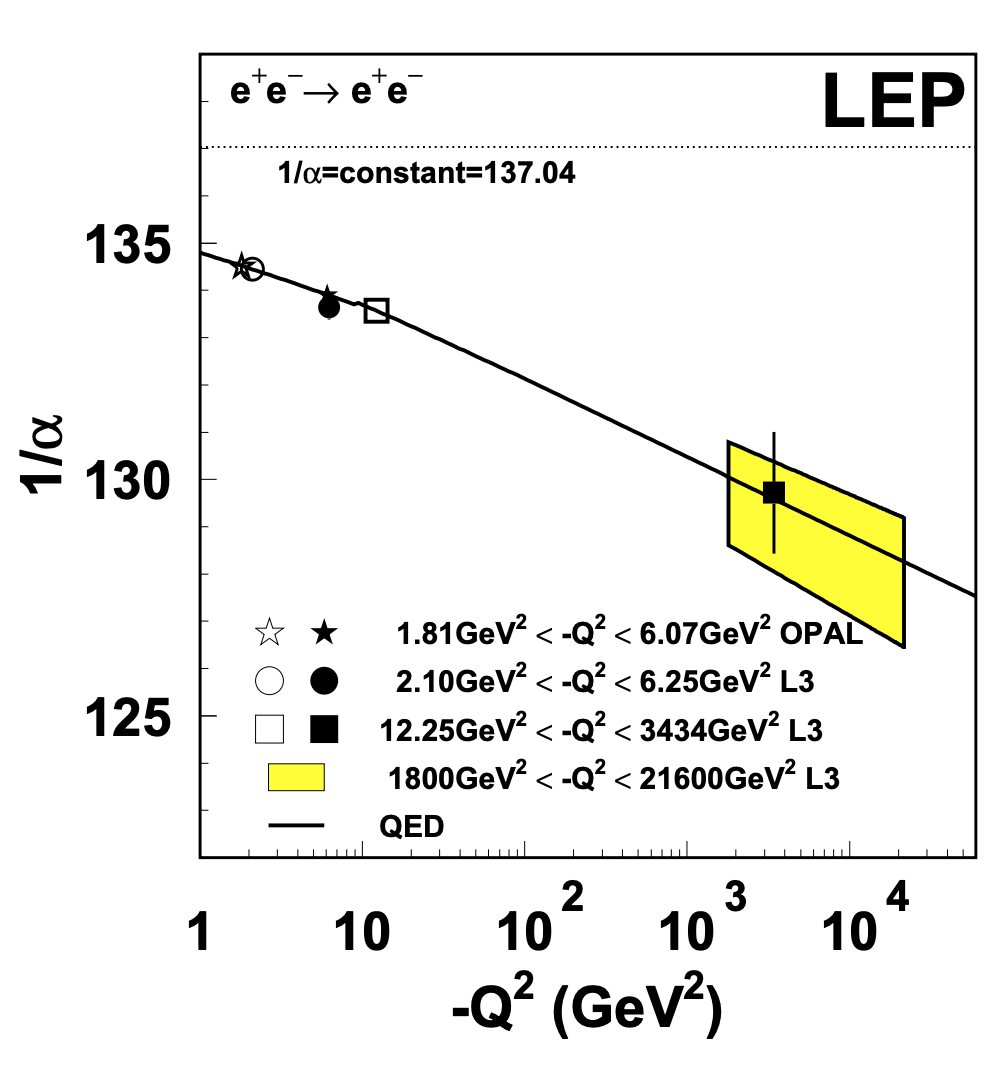
\includegraphics[width=0.39\textwidth]{figures/Phenomenology/alphaRunning.png}
   \raisebox{0.1\height}{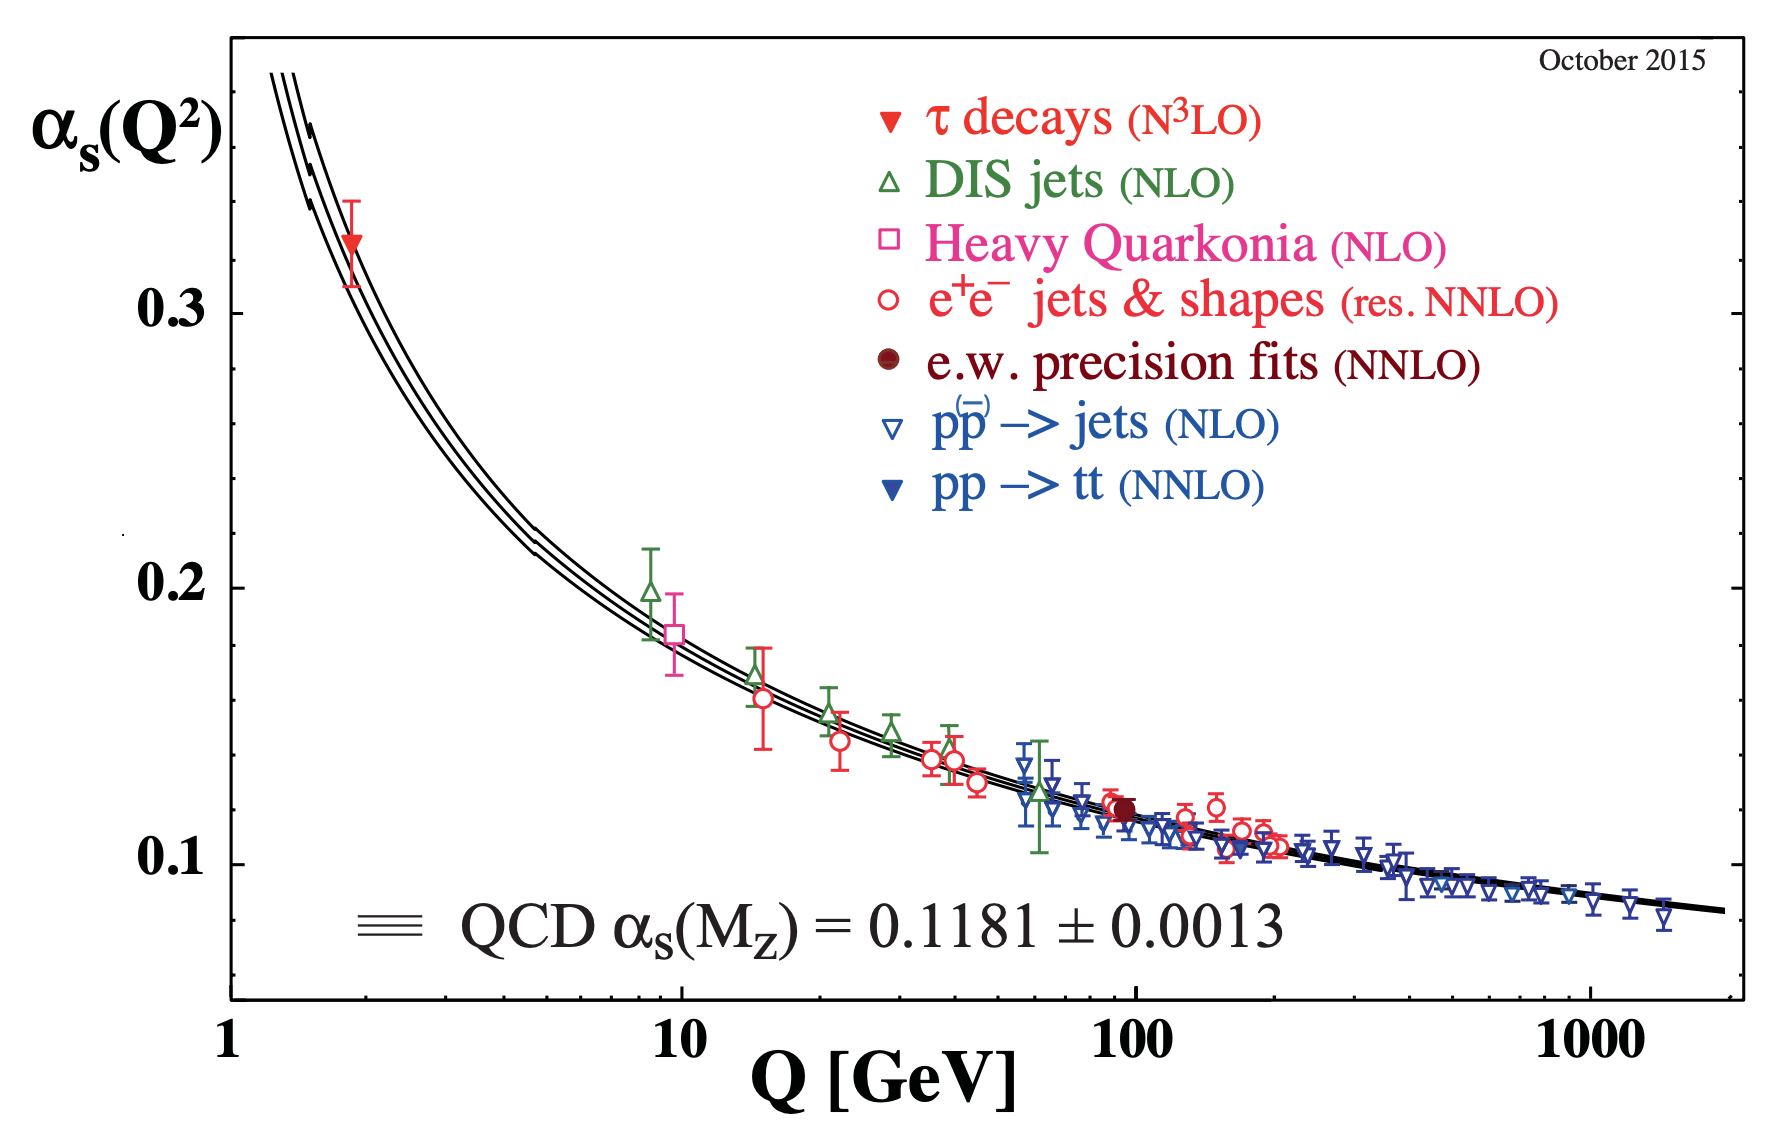
\includegraphics[width=0.59\textwidth]{figures/Phenomenology/alphasRunning.png}}
  \caption[The energy scale dependence of the effective EW and QCD couplings]{
    The energy scale dependence of the effective EW (left, reproduced from Ref.~\cite{Mele:2006ji}) 
    and QCD (right, reproduced from Ref.~\cite{Tanabashi:2018oca}) couplings. The theoretically
    predicted bands and discrete points established experimentally are shown.
  }
\end{figure}

The energy dependence of the effective coupling constants for the 
EW and QCD theories are shown in Fig.~\ref{fig:couplings}.
As shown, the nature of the $\SUthree$ and $\SUtwo$ forces leads to a striking difference
in energy dependence between the two theories: the EW coupling strength increases
with energy, whereas the QCD coupling decreases, leading to the 
confinement of quarks and gluons into bound states, such as the proton and neutron,
at low energies. At the energy scale probed in LHC collisions, the QCD coupling is
sufficiently small for perturbative calculations, however, higher-order corrections
are often significant. The scale dependence of the EW coupling is minimal, so
higher-order EW corrections are often not essential to accurate calculations.
Perturbative calculations are discussed in more detail in Chapter~\ref{ch:simulation}.

\section{The \WZ production at the LHC}

This thesis is based on an analysis of $\pp$ collisions. At low energy, the proton can be viewed as a bound state
of the quarks $\cPqu\cPqu\cPqd$. However, at higher energy, the content of the proton
appears more complex. High-energy quarks can radiate gluons, which can split to $\cPq\cPaq$ pairs.
In the high-energy LHC collisions, the proton is a source of gluons, and
all flavors of quarks but the heaviest, the top quark.
Therefore, the initial state of fundamental particles in the interactions studied at the LHC is always
composed of quarks and gluons, collectively dubbed ``partons.'' The energy of the colliding 
protons is controlled, but the flavor and energy of the interacting partons can only 
be inferred based on these properties, as discussed in Chapter~\ref{ch:simulation}.

The dominant modes of $\pp\to\WZ3\ell\nu$ production are shown in Fig.~\ref{fig:wz3lfeynman}.
Equivalent diagrams are possible with the $\PW$ and $\PZ$ bosons coupling
to quarks, or the $\PZ$ boson to neutrinos. Many aspects of the processes are similar,
and it is often justified to treat the $\pp\to\WZ$ and $\WZ$ decay to leptons, neutrinos,
or quarks separately. For this reason, we refer to ``$\WZ$ production,'' keeping in mind
that the $\PW$ and $\PZ$ bosons have an extremely short lifetime and are only observable
via their decay products. The results in this thesis exploit the leptonic decay channels,
$\WZ\to\EE\mu\nu_{\mu}$ and $\WZ\to\MM\mathrm{e}\nu_{e}$.

Studies of $\WZ$ production at the LHC provide an important test of the SM.
As shown in Fig.~\ref{}, the process is sensitive to the charged $\PW\PZ\PZ$
coupling, which arises due to the non-Abelian nature of the electroweak
theory, and is exactly predicted in the SM~\ref{}. Additional charged
resonances, or other modifications of the \EW sector of the SM, would
modify this process and adjust the rate. Moreover, the process is known
to be sensitive to higher-order corrections~\ref{}. Measuring this process
with sufficient accuracy to test state-of-the-art calculation, and to 
determine consistency with the SM or uncover hints of new physics, is
of great interest to the LHC experimental program.

As mentioned in the previous section, it is often advantageous to consider
measurements inclusive in the number of hadronic particles. It is possible, however,
to make exclusive measurements, provided that we are careful in how we associate
the number of hadronic objects objects to the number of partons in a Feynamn diagram.
The solution is to cluster the partons, or hadrons, using algorithms that are
well-behaved for low energy partons. We refer to these clustered hadronic objects as
``jets,'' (\jet) and a close correspondence between experimental measurements and theoretical
predictions has been demonstrated for several so-called jet-clustering algorithms.
The specific algorithms used in this analysis will be discussed in Chapter~\ref{ch:reconstruction}.
While it is often useful to relate the $\WZ+2$ partons calculation and the $\WZ+2$ jets (\WZjj)
experimental state, it is important to note that the relationship is most appropriate
when using a common jet clustering algorithm.

The focus of this thesis is the process
$\pp\to\WZjj$, an important subcomponent of the inclusive $\pp\to\WZ$ process
Here, and throughout this thesis, $\WZjj$ refers to $\WZ$ production,
with leptonic decays,
associated with at least two jets in the event, e.g., a final state of $3\ell\nu\jet\jet$.
The dominant contribution to the $\WZjj$ state is a higher-order correction to the 
diagrams of Fig.~\ref{fig:wz3lfeynman}, where gluons are radiated from the incoming
quark lines, as shown in Fig~\ref{fig:FeynmanDiagrams} (left). Because of the additional
QCD vertices, these diagrams contribute to the \WZjj state at $\mathcal{O}(\alpha_s^{2}\alpha^{2})$,
compared with $\mathcal{O}(\alpha_s^{0}\alpha^{2})$ for the dominant contributions to the $\pp\to\WZ$
process. At this order, contributions from $\cPq\cPg$ and $\cPg\cPg$ initial
states also contribute, slightly enhancing the total $\WZjj$ production rate.
In addition, another contribution at $\mathcal{O}(\alpha_s^{0})$ emerges, of
order $\mathcal{O}(\alpha_s^{4})$. 
The subclass of processes with only EW couplings at tree level has a rich
and important phenomenology.
It includes contributions from vector boson scattering (VBS), 
where vector bosons are radiated from the incoming quarks before interacting,
as illustrated in Fig.~\ref{fig:feynmanDiagrams}~(left). 
The VBS processes form a distinct experimental signature characterized by 
the $\PW$ and $\PZ$ bosons with two forward, 
high-momentum jets, arising from the hadronization of two quarks. 
$\mathcal{O}(\alpha^4)$, referred to as EW-induced \WZjj production, or simply \EWWZ production. 
The previously discussed contributions to the \WZjj state that proceed via QCD 
radiation of partons from are referred to as QCD-induced WZjj production (or \QCDWZ).

\begin{figure}[htbp]
  \centering
   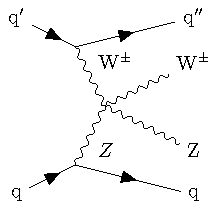
\includegraphics[page=1,width=0.25\textwidth]{figures/FeynmanDiagrams/feynmanVBS.pdf}
   \includegraphics[page=2,width=0.25\textwidth]{figures/FeynmanDiagrams/feynmanVBS.pdf}
   \includegraphics[page=3,width=0.25\textwidth]{figures/FeynmanDiagrams/feynmanVBS.pdf}
  \caption{Representative Feynman diagrams for \WZjj production in the SM and BSM. 
  EW-induced WZ production includes quartic interactions (a) of the vector bosons.
  New physics in the EW sector modifying the quartic coupling 
  can be parameterized in terms of dimension-eight effective field theory operators (b).
  Specific models modifying this interaction include those predicting charged Higgs bosons (c).
  }
 \label{fig:feynmanDiagrams}
\end{figure}

\section{Probing the electroweak sector through vector boson scattering}

As illustrated in Fig.~\ref{fig:feynmanDiagrams} (right), \EWWZ production 
is sensitive to the quartic couplings of the vector bosons. In addition,




Why is the quartic coupling interesting?

The historical significance of the WZ vector boson scattering process

\subsection{Additional Higgs bosons and the Georgi-Machacek model}

In the SM, EWSB is realized by a single isospin doublet scalar field.
This field is sufficient to give mass to the $\PW$ and $\cPZ$
bosons, while resulting in the scalar $\PH$ boson, consistent with the observed
boson with $m_{\PH} = 125\GeV$.  Especially given the complexity of the fermion sector
of the SM, it is natural to ask if the universe contains a more complex
structure of scalar fields than the single doublet. 
However, SM extensions by arbitrary \SUtwo scalar fields 
are high constrained by the parameter $\rho \equiv m_\PW^2/m_\PZ^w\cos^2\theta$,
experimentally established to be very close to 1~\cite{}.
For a theory with $n$ scalar multiplets
$\phi_i$, with weak Isospin $I_i$, weak hypercharge $Y_i$, and vacuum expectation
value $v_i$, $\rho$ is given defined in terms of the quantum numbers of the fields
by the following expression at tree level~\cite{Branco:2011iw}
\begin{equation}
  \rho = \sum_{i = 1}^{n} \frac{I_i(I_i+1) - \frac{1}{4}Y_i^2}
              {\frac{1}{2}Y_i^2 v_i} \,,
  \label{eq:rho}
\end{equation}
Extending the scalar sector of the SM by two rather than one doublet satisfies
this expression. This model, known as the Two-Higgs-doublet model (2HDM), has
been extensively studied, in part because the scalar sector of SUSY has this form.
The 2HDM gives rise to a heavy Higgs boson, a pseudoscalar Higgs boson, and 
charged Higgs bosons $\PH^{\pm}$ in addition to a light SM-like Higgs boson.
In this model, the $\PH^{\pm}$ bosons coupling strongly to the leptons,
and decays to bosons are strongly suppressed in the mass range probed by the LHC~\cite{Arhrib:2016wpw}.

An alternative extension of the Higgs sector of the SM that satisfies experimental
constraints on $\rho$ was first proposed by Georgi and Machecek~\cite{Georgi:1985nv}.
In the Georgi Machacek (GM) model, the Higgs sector is extended by a real 
triplet with $Y=0$ and 
a complex triplet with $Y=2$ in addition to the usual SM doublet ($Y =1$). 
After EWSB, this leads to a rich Higgs sector with intriguing phenomenology.
The Higgs sector of the GM has ten physical states that are organized based
on their transformation properties under the approximate global $\SUtwo$ symmetry
of the scalar fields, referred to as custodial symmetry. There are two singlets,
one of which is associated with the observed Higgs boson, a triplet, and 
a fiveplet ($\PH_5^{++}$,$\PH_5^{+}$,$\PH_5^{0}$,$\PH_5^{-}$,$\PH_5^{--}$) that
is fermiophobic. If the mass of the triplet states is greater than the
mass of the fiveplet, the only production mechanism for $\PH^{\pm}$ at the LHC
is vector boson fusion (VBF). The production cross section is proportional to the variable
$s_{\PH}^2 \equiv \sin^2{\theta_{\PH}}$, where $\sin{\theta_{\PH}} = 2\sqrt{2}v_{\chi}/v$,
the ratio
of the vacuum expectation value (vev) of the triplet fields to the SM vev. 
The $\WZjj$ state probed in this thesis is well-suited for further probes of this model, 
which is significantly less constrained than those charged Higgs with predominantly
leptonic decays.

\subsection{Generalizing new $\WWZZ$ interactions with effective field theory}

If new physics is present VBS WZ production 

\section{Previous results}

\subsection{Measurements of \WZ production}
The inclusive \WZ production cross section in \pp collisions 
has been measured in the leptonic decay modes by the ATLAS and CMS Collaborations 
at 7, 8, and $13\TeV$~\cite{Aad:2012twa,Aad:2016ett,Aaboud:2016yus,Aaboud:2019gxl,Khachatryan:2016tgp,Khachatryan:2016poo}, 
A summary of these measurements is 
shown in Fig.~\ref{fig:WZxsecSqrts}. The summarized experimental results are obtained
by measuring $\pp\to\WZ\to\ell\ell\ell'\nu$ process, corrected for the 
independently-measured leptonic branching ratios (the percentage of events with
$\PW\to\ell\nu$ and $\PZ\to\ell\ell$ to all other decay channels), to obtain a total
rate for the process $\pp\to\WZ$. Theoretical predictions are shown at 
next-to-leading order (NLO) in QCD, in which all contributions to the process 
up to $\alpha^{2}\alpha_s$ are considered in the calculation,
and at next-to-next-to-leading order (NNLO), which considers contributions up 
to $\alpha^{2}\alpha_s^{2}$. The predictions are obtained using the programs
MCFM~\cite{Campbell:2011bn,Campbell:2015qma} and MATRIX~\cite{Grazzini:2016swo,Grazzini:2017mhc}.
The data exhibit a slight preference for the higher-order prediction, demonstrating
the importance of both high-precision measurements and calculations.

\begin{figure}[htbp]
  \centering
   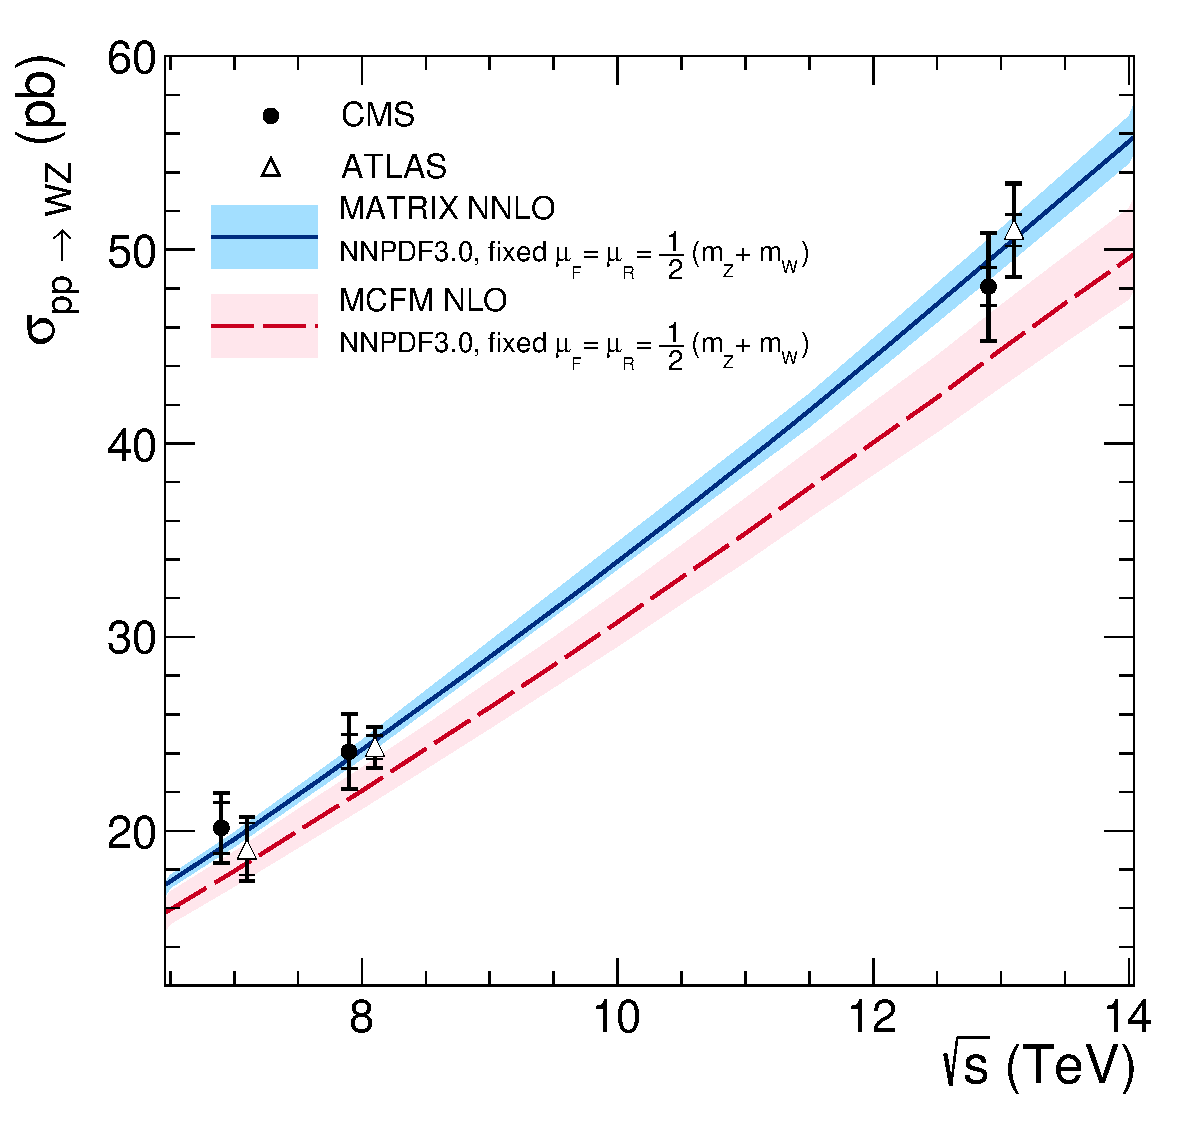
\includegraphics[width=0.8\textwidth]{figures/Phenomenology/WZCrossSection_preliminary_2019-02-23.pdf}
  \caption{
    The measured $\pp\to\WZ$ production cross sections at 7, 8, and 13\TeV compared with
    theoretical predictions at NLO and NNLO in QCD.
        }
 \label{fig:WZxsecSqrts}
\end{figure}


\subsection{Measurements of $\WZjj$ production and electroweak \WZ production}

Fig.~\ref{fig:WZnJets} shows the distribution of the number of jets associated with
the selected $\ell\ell\ell'\nu$ state in data collected by the CMS experiment
in 2015. This analysis, the first measurement of the $\WZ$ process at 13\TeV,
was a critical first towards the $\WZjj$
studies presented in this thesis. The expected contribution from the $\WZ$
process, along with the estimated backgrounds, are seen to be in good agreement
with the observed data. This studies of this thesis are performed with
a higher-luminosity data set, in order to exploit the kinematics variables of the selected
jets to isolate the $\EWWZ$ and new physics contributions.

\begin{figure}[htbp]
  \centering
   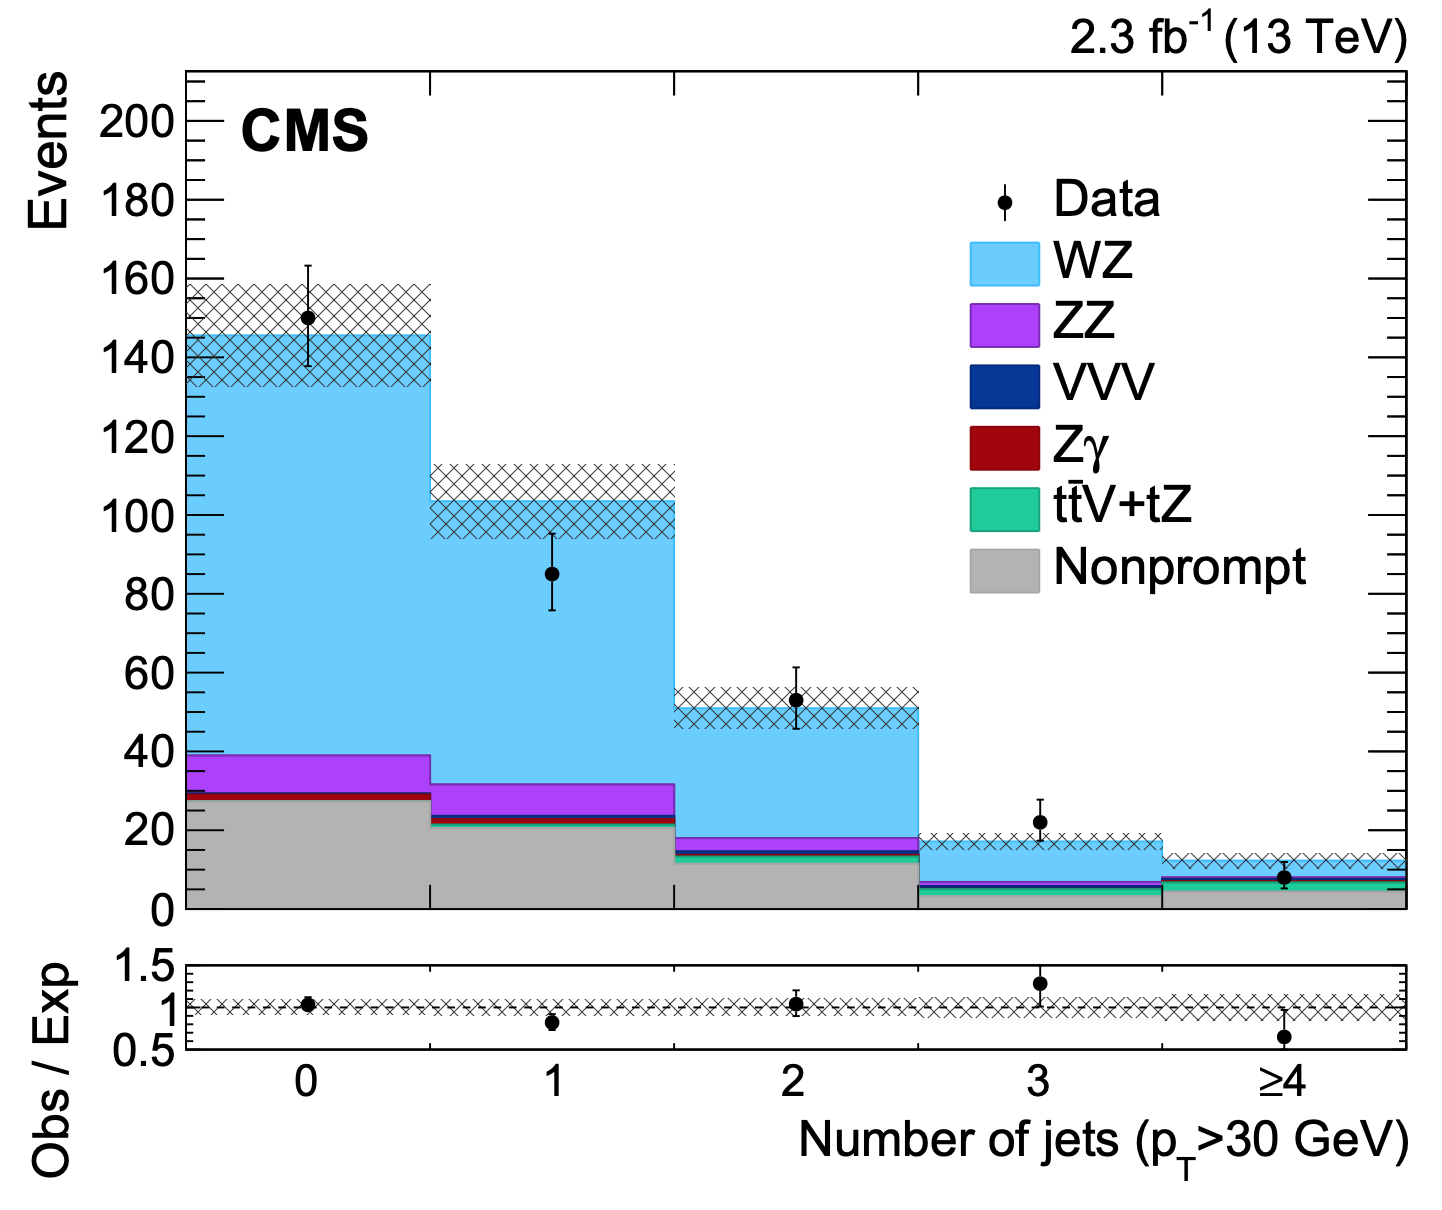
\includegraphics[width=0.6\textwidth]{figures/Phenomenology/WZnJets2015.png}
  \caption{
    The number of jets in selected $\ell\ell\ell'\nu$ events
    for the observed data and the expected $\WZ$ signal and background 
    contributions using 2.3\fbinv of data collected by the CMS experiment in
    2015~\cite{Khachatryan:2016tgp}.
        }
 \label{fig:WZnJets}
\end{figure}

The first studies of VBS production of pairs of massive vector 
bosons---termed diboson production, or VV production, where $\text{V}=\PW,\PZ$---were 
performed using in the $\pp\to\Wpm\Wpm\to\ell^{\pm}\nu\ell'^{\pm}\nu'$
channel at 8\TeV~\cite{Khachatryan:2014sta,Aad:2014zda,Aaboud:2016ffv}.
This channel is advantageous at the LHC, because, contrary to all other VV states,
the {\EW}-induced production dominates the QCD-induced production. The first
measurement of VBS production of a massive VV state with statistical significance
exceeding 3.0 standard deviations ($\sigma$) is presented by the ATLAS Collaboration 
in the analysis of Ref.~\cite{Aad:2014zda}.
The \EWWZ production was also studied at 8\TeV by the ATLAS Collaboration,
which places upper limits on the production cross section in Ref.~\cite{Aad:2016ett},
and the CMS Collaboration, which reports a \WZjj cross section in a region
sensitive to \EWWZ production in Ref.~\cite{Khachatryan:2014sta}.

Studies of \EW $\Wpm\Wpm$ have recently been performed by the CMS and ATLAS Collaborations at 
13\TeV~\cite{Sirunyan:2017ret,ATLAS-CONF-2018-030}.
The first measurement of \EW VV production with a statistical significance greater than 5 standard 
deviations, considered the standard for discovery of new processes by the experimental particle 
physics community, is presented by the CMS Collaboration in Ref.~\cite{Sirunyan:2017fvv}. A subsequent study
performed by the ATLAS Collaboration~\cite{ATLAS-CONF-2018-030} reports a comparable observation for the process.
The first study of the \EW VV production with a $\PZ$ boson was performed in the $\pp\to\ZZ$ channel
by the CMS Collaboration~\cite{Sirunyan:2017jej}. The observed statistical significance of the 
measurement is $2.7\sigma$ with $1.9\sigma$ expected in the SM.

The analysis of this thesis, submitted for publication to the journal \emph{Physics Letters B}~\cite{Sirunyan:2019ksz},
is the first study of \EWWZ production performed by the CMS.
An analysis using a comparable data set of $\pp$ collisions at 13\TeV
has also been submitted to the journal \emph{Physics Letters B} by the ATLAS collaboration~\cite{Aaboud:2018ddq}.
The ATLAS analysis reports and observation of the \EWWZ process with observed statistical significance of
$5.3\sigma$, with $3.4\sigma$ expected in the SM.


\subsection{Measurements of the quartic \WWZZ coupling}

and limits on anomalous triple gauge couplings~\cite{Hagiwara:1989mx} are presented in Refs.~\cite{Aad:2016ett,Khachatryan:2016poo}. 
Constraints on anomalous quartic gauge couplings (aQGC)~\cite{Eboli:2006wa}
are presented by the ATLAS Collaboration at $8\TeV$ in Ref.~\cite{Aad:2016ett}. 

Limits from SS WW @ 13 TeV, and ZZ. Triple W production from ATLAS?

\begin{figure}[htbp]
  \centering
   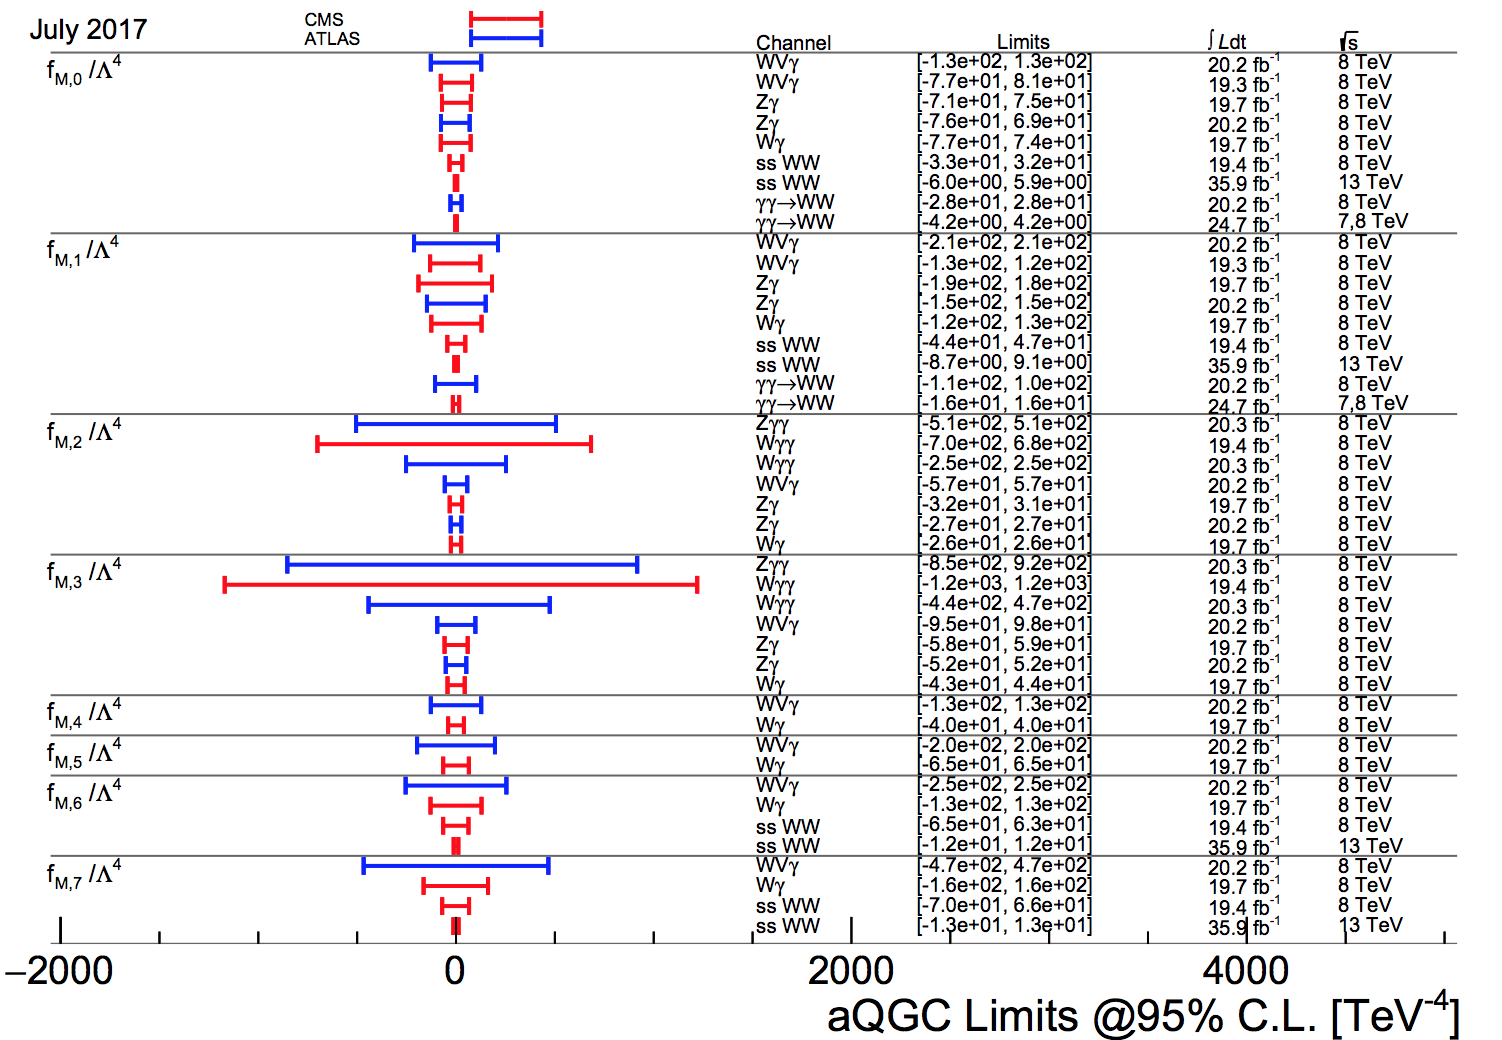
\includegraphics[width=0.95\textwidth]{figures/Phenomenology/FM0_limits_Jun2017.png}
  \caption{
    Constraints on the parameters f$_{\text{Mi}}/\Lambda^4$ for dimension-8 EFT
    operators from the CMS and ATLAS experiments.
        }
 \label{fig:}
\end{figure}

\subsection{Measurements of charged Higgs production via vector boson fusion}

The first studies of the production of charged Higgs bosons produced via VBF
and decaying to $\WZ$ at the LHC were performed by the ATLAS Collaboration
at 8~\TeV~\cite{Aad:2015nfa}. The analysis exploited the decay channel
$\Wpm\to\cPq\cPaq'$ and $\PZ\to\ell\ell'$ (where $\ell=\mathrm{e},\mu$)
to place the first direct production constraints on the GM model, as well as model-independent
limits on the production of a narrow-width charged Higgs produced via VBF.
The CMS Collaboration extended this analysis with a study of the VBF $\PH^{\pm}$ 
using $15.2\fbinv$ of data collected at
$13\TeV$, exploiting the leptonic decay channel $\WZ\to\ell\ell\ell'\nu$~\cite{Sirunyan:2017sbn}.
The ATLAS Collaboration recently performed an analysis of the same channel
using the data delivered by the LHC in 2016, corresponding to $36.1\fbinv$~\cite{Aaboud:2018ohp},
extending the constraints of the previous CMS analysis.
A local excess of events over the SM prediction was at a resonance mass of
around 450\GeV was suggested by this analysis, with a global significance
of $1.9\sigma$ when interpreted in the GM model.
The analysis presented in this thesis extends the results of the previous CMS study, 
and is comparable to the recent study by the ATLAS Collaboration.

\begin{figure}[htbp]
  \centering
   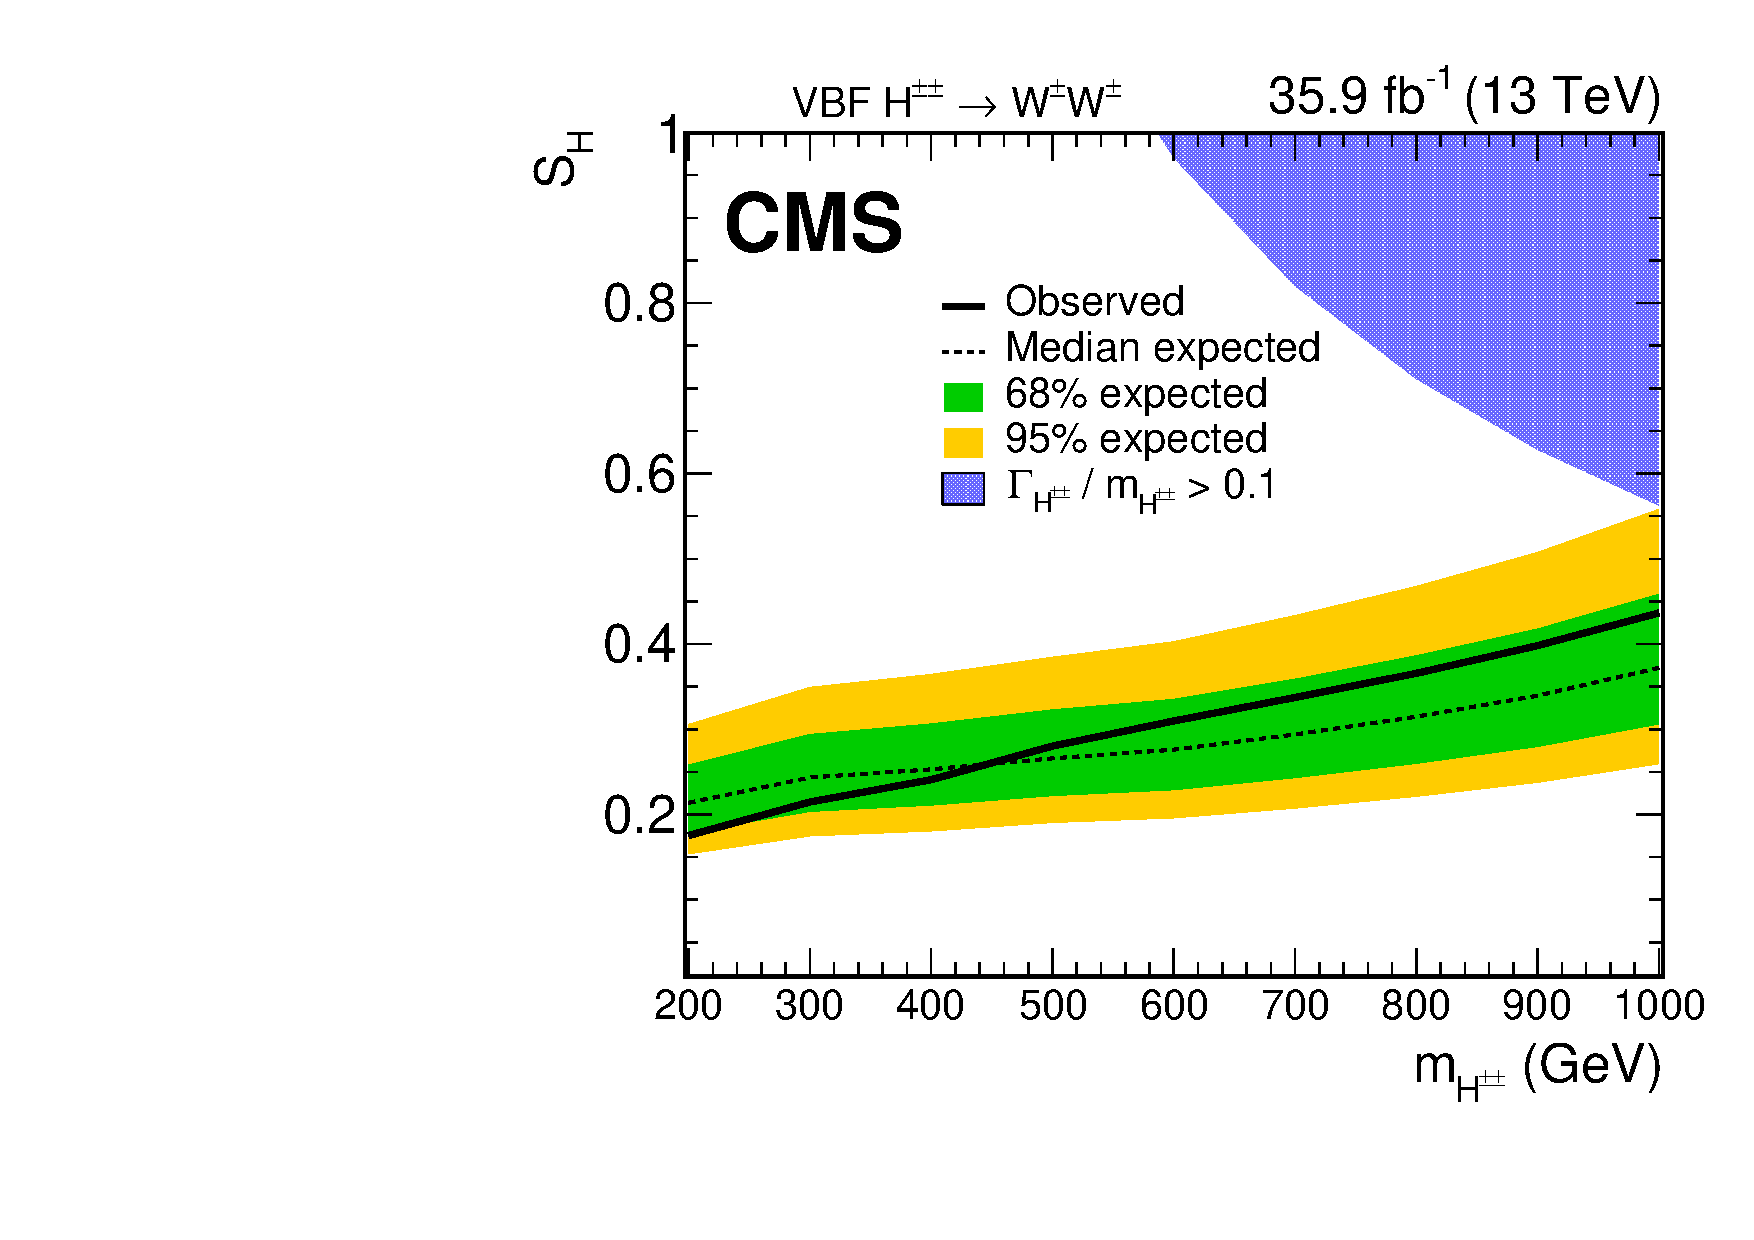
\includegraphics[width=0.44\textwidth]{figures/Phenomenology/CMS-SMP-17-004_Figure_003-b.pdf}
   \raisebox{0.08\height}{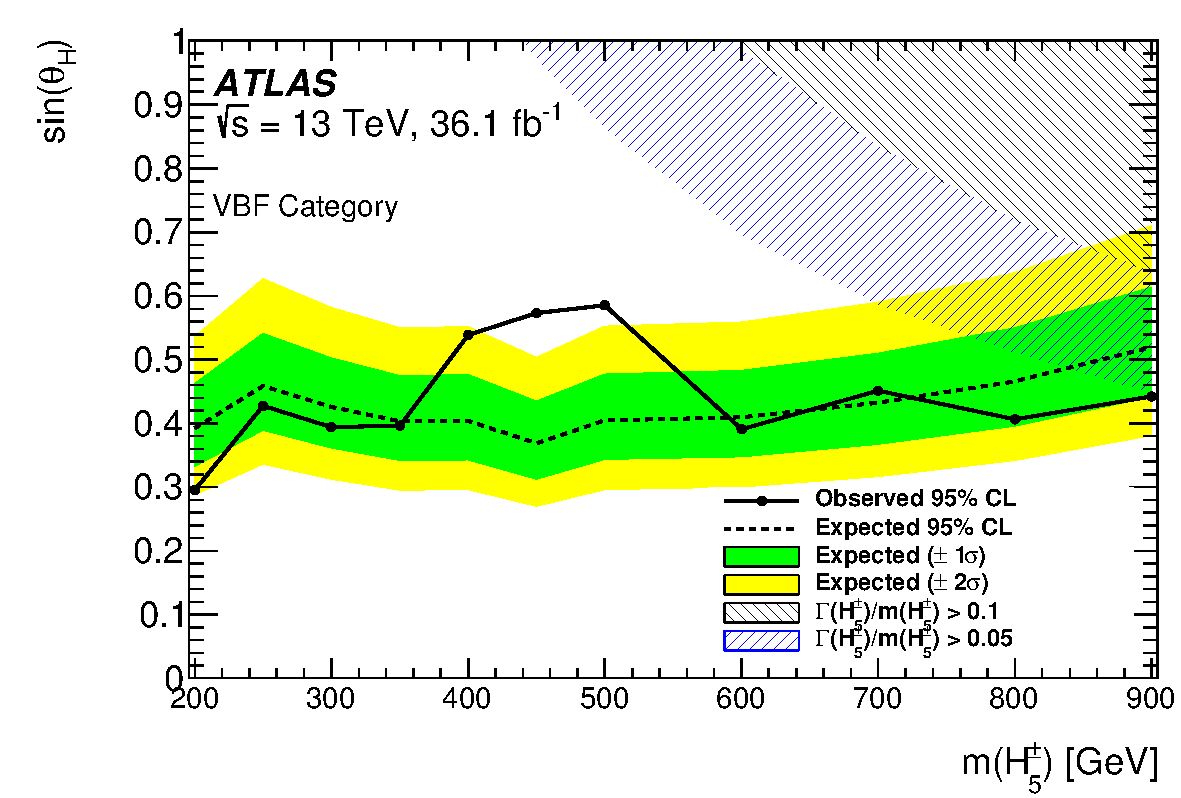
\includegraphics[width=0.54\textwidth]{figures/Phenomenology/ATLAS-EXOT-2016-11_fig_07b.pdf}}
  \caption{
    Limits on production of doubly charged (left, from Ref.~\cite{Sirunyan:2017ret}) 
    and charged Higgs bosons (right, from Ref.~\cite{Aaboud:2018ohp}) in the H5plane defined by the GM model.
        }
 \label{fig:GeorgiMachacekLimits}
\end{figure}

Members of the custodial fiveplet in the GM model have a common mass $m_{\PH^{5}}$.
Therefore, limits on doubly charged Higgs bosons $\PH^{\pm\pm}$
are complementary to those obtained for $\PH^{\pm}$ production when interpreted under this model. 
The ATLAS and CMS
Collaborations have studied $\PH^{\pm\pm}$ production with decays to same-sign
$\PW$ bosons at 8\TeV~\cite{Aad:2014zda,Khachatryan:2014sta}, and the CMS Collaboration has presented
constraints at 13\TeV~\cite{Sirunyan:2017ret}. 
The constraints on the VBF production of $\PH^{\pm}$ in the GM model from Ref.~\cite{Aaboud:2018ohp}
and for $\PH^{\pm\pm}$ from Ref.~\cite{Sirunyan:2017ret} are shown in Fig.~\ref{fig:GeorgiMachacekLimits}.
The limits are presented in terms of $s_{\PH}^2$ and the mass of the $\PH^{\pm}$ or $\PH^{\pm\pm}$
boson, which defines the ``H5plane'' proposed by the LHC Higgs Cross Sections Working Group in Ref.~\cite{deFlorian:2016spz}.
The H5plane is defined with the assumptions that the triplet mass is greater than the 
fiveplet mass and that the parameters of the model allow perturbative calculations. 
Additional constraints on the GM model arise from studies of $\cPqb$ hadron decay
and heavy Higgs boson searches, which are impacted by contributions from additional
Higgs bosons contributing in loop diagrams, but these constraints are exceeded
by the direct measurements discussed here. Global fits of the direct and indirect
constraints on the GM model can be found in Ref.~\cite{Chiang:2018cgb}.

